
% Default to the notebook output style

    


% Inherit from the specified cell style.




    
\documentclass{article}

    
    \usepackage{float}
    \usepackage{graphicx} % Used to insert images
    \usepackage{adjustbox} % Used to constrain images to a maximum size 
    \usepackage{color} % Allow colors to be defined
    \usepackage{enumerate} % Needed for markdown enumerations to work
    \usepackage{geometry} % Used to adjust the document margins
    \usepackage{amsmath} % Equations
    \usepackage{amssymb} % Equations
    \usepackage{eurosym} % defines \euro
    \usepackage[mathletters]{ucs} % Extended unicode (utf-8) support
    \usepackage[utf8x]{inputenc} % Allow utf-8 characters in the tex document
    \usepackage{fancyvrb} % verbatim replacement that allows latex
    \usepackage{grffile} % extends the file name processing of package graphics 
                         % to support a larger range 
    % The hyperref package gives us a pdf with properly built
    % internal navigation ('pdf bookmarks' for the table of contents,
    % internal cross-reference links, web links for URLs, etc.)
    \usepackage{hyperref}
    \usepackage{longtable} % longtable support required by pandoc >1.10
    \usepackage{booktabs}  % table support for pandoc > 1.12.2
    \usepackage{ulem} % ulem is needed to support strikethroughs (\sout)
    

    
    
    \definecolor{orange}{cmyk}{0,0.4,0.8,0.2}
    \definecolor{darkorange}{rgb}{.71,0.21,0.01}
    \definecolor{darkgreen}{rgb}{.12,.54,.11}
    \definecolor{myteal}{rgb}{.26, .44, .56}
    \definecolor{gray}{gray}{0.45}
    \definecolor{lightgray}{gray}{.95}
    \definecolor{mediumgray}{gray}{.8}
    \definecolor{inputbackground}{rgb}{.95, .95, .85}
    \definecolor{outputbackground}{rgb}{.95, .95, .95}
    \definecolor{traceback}{rgb}{1, .95, .95}
    % ansi colors
    \definecolor{red}{rgb}{.6,0,0}
    \definecolor{green}{rgb}{0,.65,0}
    \definecolor{brown}{rgb}{0.6,0.6,0}
    \definecolor{blue}{rgb}{0,.145,.698}
    \definecolor{purple}{rgb}{.698,.145,.698}
    \definecolor{cyan}{rgb}{0,.698,.698}
    \definecolor{lightgray}{gray}{0.5}
    
    % bright ansi colors
    \definecolor{darkgray}{gray}{0.25}
    \definecolor{lightred}{rgb}{1.0,0.39,0.28}
    \definecolor{lightgreen}{rgb}{0.48,0.99,0.0}
    \definecolor{lightblue}{rgb}{0.53,0.81,0.92}
    \definecolor{lightpurple}{rgb}{0.87,0.63,0.87}
    \definecolor{lightcyan}{rgb}{0.5,1.0,0.83}
    
    % commands and environments needed by pandoc snippets
    % extracted from the output of `pandoc -s`
    \providecommand{\tightlist}{%
      \setlength{\itemsep}{0pt}\setlength{\parskip}{0pt}}
    \DefineVerbatimEnvironment{Highlighting}{Verbatim}{commandchars=\\\{\}}
    % Add ',fontsize=\small' for more characters per line
    \newenvironment{Shaded}{}{}
    \newcommand{\KeywordTok}[1]{\textcolor[rgb]{0.00,0.44,0.13}{\textbf{{#1}}}}
    \newcommand{\DataTypeTok}[1]{\textcolor[rgb]{0.56,0.13,0.00}{{#1}}}
    \newcommand{\DecValTok}[1]{\textcolor[rgb]{0.25,0.63,0.44}{{#1}}}
    \newcommand{\BaseNTok}[1]{\textcolor[rgb]{0.25,0.63,0.44}{{#1}}}
    \newcommand{\FloatTok}[1]{\textcolor[rgb]{0.25,0.63,0.44}{{#1}}}
    \newcommand{\CharTok}[1]{\textcolor[rgb]{0.25,0.44,0.63}{{#1}}}
    \newcommand{\StringTok}[1]{\textcolor[rgb]{0.25,0.44,0.63}{{#1}}}
    \newcommand{\CommentTok}[1]{\textcolor[rgb]{0.38,0.63,0.69}{\textit{{#1}}}}
    \newcommand{\OtherTok}[1]{\textcolor[rgb]{0.00,0.44,0.13}{{#1}}}
    \newcommand{\AlertTok}[1]{\textcolor[rgb]{1.00,0.00,0.00}{\textbf{{#1}}}}
    \newcommand{\FunctionTok}[1]{\textcolor[rgb]{0.02,0.16,0.49}{{#1}}}
    \newcommand{\RegionMarkerTok}[1]{{#1}}
    \newcommand{\ErrorTok}[1]{\textcolor[rgb]{1.00,0.00,0.00}{\textbf{{#1}}}}
    \newcommand{\NormalTok}[1]{{#1}}
    
    % Additional commands for more recent versions of Pandoc
    \newcommand{\ConstantTok}[1]{\textcolor[rgb]{0.53,0.00,0.00}{{#1}}}
    \newcommand{\SpecialCharTok}[1]{\textcolor[rgb]{0.25,0.44,0.63}{{#1}}}
    \newcommand{\VerbatimStringTok}[1]{\textcolor[rgb]{0.25,0.44,0.63}{{#1}}}
    \newcommand{\SpecialStringTok}[1]{\textcolor[rgb]{0.73,0.40,0.53}{{#1}}}
    \newcommand{\ImportTok}[1]{{#1}}
    \newcommand{\DocumentationTok}[1]{\textcolor[rgb]{0.73,0.13,0.13}{\textit{{#1}}}}
    \newcommand{\AnnotationTok}[1]{\textcolor[rgb]{0.38,0.63,0.69}{\textbf{\textit{{#1}}}}}
    \newcommand{\CommentVarTok}[1]{\textcolor[rgb]{0.38,0.63,0.69}{\textbf{\textit{{#1}}}}}
    \newcommand{\VariableTok}[1]{\textcolor[rgb]{0.10,0.09,0.49}{{#1}}}
    \newcommand{\ControlFlowTok}[1]{\textcolor[rgb]{0.00,0.44,0.13}{\textbf{{#1}}}}
    \newcommand{\OperatorTok}[1]{\textcolor[rgb]{0.40,0.40,0.40}{{#1}}}
    \newcommand{\BuiltInTok}[1]{{#1}}
    \newcommand{\ExtensionTok}[1]{{#1}}
    \newcommand{\PreprocessorTok}[1]{\textcolor[rgb]{0.74,0.48,0.00}{{#1}}}
    \newcommand{\AttributeTok}[1]{\textcolor[rgb]{0.49,0.56,0.16}{{#1}}}
    \newcommand{\InformationTok}[1]{\textcolor[rgb]{0.38,0.63,0.69}{\textbf{\textit{{#1}}}}}
    \newcommand{\WarningTok}[1]{\textcolor[rgb]{0.38,0.63,0.69}{\textbf{\textit{{#1}}}}}
    
    
    % Define a nice break command that doesn't care if a line doesn't already
    % exist.
    \def\br{\hspace*{\fill} \\* }
    % Math Jax compatability definitions
    \def\gt{>}
    \def\lt{<}
    % Document parameters
    \title{Review of Statistical Analysis of Numerical Preclinical Radio-biological Data}
    \author{Raaz Dwivedi,  Antonio Iannopollo and Jiancong Chen}
    
    
    

    % Pygments definitions
    
\makeatletter
\def\PY@reset{\let\PY@it=\relax \let\PY@bf=\relax%
    \let\PY@ul=\relax \let\PY@tc=\relax%
    \let\PY@bc=\relax \let\PY@ff=\relax}
\def\PY@tok#1{\csname PY@tok@#1\endcsname}
\def\PY@toks#1+{\ifx\relax#1\empty\else%
    \PY@tok{#1}\expandafter\PY@toks\fi}
\def\PY@do#1{\PY@bc{\PY@tc{\PY@ul{%
    \PY@it{\PY@bf{\PY@ff{#1}}}}}}}
\def\PY#1#2{\PY@reset\PY@toks#1+\relax+\PY@do{#2}}

\expandafter\def\csname PY@tok@gd\endcsname{\def\PY@tc##1{\textcolor[rgb]{0.63,0.00,0.00}{##1}}}
\expandafter\def\csname PY@tok@gu\endcsname{\let\PY@bf=\textbf\def\PY@tc##1{\textcolor[rgb]{0.50,0.00,0.50}{##1}}}
\expandafter\def\csname PY@tok@gt\endcsname{\def\PY@tc##1{\textcolor[rgb]{0.00,0.27,0.87}{##1}}}
\expandafter\def\csname PY@tok@gs\endcsname{\let\PY@bf=\textbf}
\expandafter\def\csname PY@tok@gr\endcsname{\def\PY@tc##1{\textcolor[rgb]{1.00,0.00,0.00}{##1}}}
\expandafter\def\csname PY@tok@cm\endcsname{\let\PY@it=\textit\def\PY@tc##1{\textcolor[rgb]{0.25,0.50,0.50}{##1}}}
\expandafter\def\csname PY@tok@vg\endcsname{\def\PY@tc##1{\textcolor[rgb]{0.10,0.09,0.49}{##1}}}
\expandafter\def\csname PY@tok@vi\endcsname{\def\PY@tc##1{\textcolor[rgb]{0.10,0.09,0.49}{##1}}}
\expandafter\def\csname PY@tok@mh\endcsname{\def\PY@tc##1{\textcolor[rgb]{0.40,0.40,0.40}{##1}}}
\expandafter\def\csname PY@tok@cs\endcsname{\let\PY@it=\textit\def\PY@tc##1{\textcolor[rgb]{0.25,0.50,0.50}{##1}}}
\expandafter\def\csname PY@tok@ge\endcsname{\let\PY@it=\textit}
\expandafter\def\csname PY@tok@vc\endcsname{\def\PY@tc##1{\textcolor[rgb]{0.10,0.09,0.49}{##1}}}
\expandafter\def\csname PY@tok@il\endcsname{\def\PY@tc##1{\textcolor[rgb]{0.40,0.40,0.40}{##1}}}
\expandafter\def\csname PY@tok@go\endcsname{\def\PY@tc##1{\textcolor[rgb]{0.53,0.53,0.53}{##1}}}
\expandafter\def\csname PY@tok@cp\endcsname{\def\PY@tc##1{\textcolor[rgb]{0.74,0.48,0.00}{##1}}}
\expandafter\def\csname PY@tok@gi\endcsname{\def\PY@tc##1{\textcolor[rgb]{0.00,0.63,0.00}{##1}}}
\expandafter\def\csname PY@tok@gh\endcsname{\let\PY@bf=\textbf\def\PY@tc##1{\textcolor[rgb]{0.00,0.00,0.50}{##1}}}
\expandafter\def\csname PY@tok@ni\endcsname{\let\PY@bf=\textbf\def\PY@tc##1{\textcolor[rgb]{0.60,0.60,0.60}{##1}}}
\expandafter\def\csname PY@tok@nl\endcsname{\def\PY@tc##1{\textcolor[rgb]{0.63,0.63,0.00}{##1}}}
\expandafter\def\csname PY@tok@nn\endcsname{\let\PY@bf=\textbf\def\PY@tc##1{\textcolor[rgb]{0.00,0.00,1.00}{##1}}}
\expandafter\def\csname PY@tok@no\endcsname{\def\PY@tc##1{\textcolor[rgb]{0.53,0.00,0.00}{##1}}}
\expandafter\def\csname PY@tok@na\endcsname{\def\PY@tc##1{\textcolor[rgb]{0.49,0.56,0.16}{##1}}}
\expandafter\def\csname PY@tok@nb\endcsname{\def\PY@tc##1{\textcolor[rgb]{0.00,0.50,0.00}{##1}}}
\expandafter\def\csname PY@tok@nc\endcsname{\let\PY@bf=\textbf\def\PY@tc##1{\textcolor[rgb]{0.00,0.00,1.00}{##1}}}
\expandafter\def\csname PY@tok@nd\endcsname{\def\PY@tc##1{\textcolor[rgb]{0.67,0.13,1.00}{##1}}}
\expandafter\def\csname PY@tok@ne\endcsname{\let\PY@bf=\textbf\def\PY@tc##1{\textcolor[rgb]{0.82,0.25,0.23}{##1}}}
\expandafter\def\csname PY@tok@nf\endcsname{\def\PY@tc##1{\textcolor[rgb]{0.00,0.00,1.00}{##1}}}
\expandafter\def\csname PY@tok@si\endcsname{\let\PY@bf=\textbf\def\PY@tc##1{\textcolor[rgb]{0.73,0.40,0.53}{##1}}}
\expandafter\def\csname PY@tok@s2\endcsname{\def\PY@tc##1{\textcolor[rgb]{0.73,0.13,0.13}{##1}}}
\expandafter\def\csname PY@tok@nt\endcsname{\let\PY@bf=\textbf\def\PY@tc##1{\textcolor[rgb]{0.00,0.50,0.00}{##1}}}
\expandafter\def\csname PY@tok@nv\endcsname{\def\PY@tc##1{\textcolor[rgb]{0.10,0.09,0.49}{##1}}}
\expandafter\def\csname PY@tok@s1\endcsname{\def\PY@tc##1{\textcolor[rgb]{0.73,0.13,0.13}{##1}}}
\expandafter\def\csname PY@tok@ch\endcsname{\let\PY@it=\textit\def\PY@tc##1{\textcolor[rgb]{0.25,0.50,0.50}{##1}}}
\expandafter\def\csname PY@tok@m\endcsname{\def\PY@tc##1{\textcolor[rgb]{0.40,0.40,0.40}{##1}}}
\expandafter\def\csname PY@tok@gp\endcsname{\let\PY@bf=\textbf\def\PY@tc##1{\textcolor[rgb]{0.00,0.00,0.50}{##1}}}
\expandafter\def\csname PY@tok@sh\endcsname{\def\PY@tc##1{\textcolor[rgb]{0.73,0.13,0.13}{##1}}}
\expandafter\def\csname PY@tok@ow\endcsname{\let\PY@bf=\textbf\def\PY@tc##1{\textcolor[rgb]{0.67,0.13,1.00}{##1}}}
\expandafter\def\csname PY@tok@sx\endcsname{\def\PY@tc##1{\textcolor[rgb]{0.00,0.50,0.00}{##1}}}
\expandafter\def\csname PY@tok@bp\endcsname{\def\PY@tc##1{\textcolor[rgb]{0.00,0.50,0.00}{##1}}}
\expandafter\def\csname PY@tok@c1\endcsname{\let\PY@it=\textit\def\PY@tc##1{\textcolor[rgb]{0.25,0.50,0.50}{##1}}}
\expandafter\def\csname PY@tok@o\endcsname{\def\PY@tc##1{\textcolor[rgb]{0.40,0.40,0.40}{##1}}}
\expandafter\def\csname PY@tok@kc\endcsname{\let\PY@bf=\textbf\def\PY@tc##1{\textcolor[rgb]{0.00,0.50,0.00}{##1}}}
\expandafter\def\csname PY@tok@c\endcsname{\let\PY@it=\textit\def\PY@tc##1{\textcolor[rgb]{0.25,0.50,0.50}{##1}}}
\expandafter\def\csname PY@tok@mf\endcsname{\def\PY@tc##1{\textcolor[rgb]{0.40,0.40,0.40}{##1}}}
\expandafter\def\csname PY@tok@err\endcsname{\def\PY@bc##1{\setlength{\fboxsep}{0pt}\fcolorbox[rgb]{1.00,0.00,0.00}{1,1,1}{\strut ##1}}}
\expandafter\def\csname PY@tok@mb\endcsname{\def\PY@tc##1{\textcolor[rgb]{0.40,0.40,0.40}{##1}}}
\expandafter\def\csname PY@tok@ss\endcsname{\def\PY@tc##1{\textcolor[rgb]{0.10,0.09,0.49}{##1}}}
\expandafter\def\csname PY@tok@sr\endcsname{\def\PY@tc##1{\textcolor[rgb]{0.73,0.40,0.53}{##1}}}
\expandafter\def\csname PY@tok@mo\endcsname{\def\PY@tc##1{\textcolor[rgb]{0.40,0.40,0.40}{##1}}}
\expandafter\def\csname PY@tok@kd\endcsname{\let\PY@bf=\textbf\def\PY@tc##1{\textcolor[rgb]{0.00,0.50,0.00}{##1}}}
\expandafter\def\csname PY@tok@mi\endcsname{\def\PY@tc##1{\textcolor[rgb]{0.40,0.40,0.40}{##1}}}
\expandafter\def\csname PY@tok@kn\endcsname{\let\PY@bf=\textbf\def\PY@tc##1{\textcolor[rgb]{0.00,0.50,0.00}{##1}}}
\expandafter\def\csname PY@tok@cpf\endcsname{\let\PY@it=\textit\def\PY@tc##1{\textcolor[rgb]{0.25,0.50,0.50}{##1}}}
\expandafter\def\csname PY@tok@kr\endcsname{\let\PY@bf=\textbf\def\PY@tc##1{\textcolor[rgb]{0.00,0.50,0.00}{##1}}}
\expandafter\def\csname PY@tok@s\endcsname{\def\PY@tc##1{\textcolor[rgb]{0.73,0.13,0.13}{##1}}}
\expandafter\def\csname PY@tok@kp\endcsname{\def\PY@tc##1{\textcolor[rgb]{0.00,0.50,0.00}{##1}}}
\expandafter\def\csname PY@tok@w\endcsname{\def\PY@tc##1{\textcolor[rgb]{0.73,0.73,0.73}{##1}}}
\expandafter\def\csname PY@tok@kt\endcsname{\def\PY@tc##1{\textcolor[rgb]{0.69,0.00,0.25}{##1}}}
\expandafter\def\csname PY@tok@sc\endcsname{\def\PY@tc##1{\textcolor[rgb]{0.73,0.13,0.13}{##1}}}
\expandafter\def\csname PY@tok@sb\endcsname{\def\PY@tc##1{\textcolor[rgb]{0.73,0.13,0.13}{##1}}}
\expandafter\def\csname PY@tok@k\endcsname{\let\PY@bf=\textbf\def\PY@tc##1{\textcolor[rgb]{0.00,0.50,0.00}{##1}}}
\expandafter\def\csname PY@tok@se\endcsname{\let\PY@bf=\textbf\def\PY@tc##1{\textcolor[rgb]{0.73,0.40,0.13}{##1}}}
\expandafter\def\csname PY@tok@sd\endcsname{\let\PY@it=\textit\def\PY@tc##1{\textcolor[rgb]{0.73,0.13,0.13}{##1}}}

\def\PYZbs{\char`\\}
\def\PYZus{\char`\_}
\def\PYZob{\char`\{}
\def\PYZcb{\char`\}}
\def\PYZca{\char`\^}
\def\PYZam{\char`\&}
\def\PYZlt{\char`\<}
\def\PYZgt{\char`\>}
\def\PYZsh{\char`\#}
\def\PYZpc{\char`\%}
\def\PYZdl{\char`\$}
\def\PYZhy{\char`\-}
\def\PYZsq{\char`\'}
\def\PYZdq{\char`\"}
\def\PYZti{\char`\~}
% for compatibility with earlier versions
\def\PYZat{@}
\def\PYZlb{[}
\def\PYZrb{]}
\makeatother


    % Exact colors from NB
    \definecolor{incolor}{rgb}{0.0, 0.0, 0.5}
    \definecolor{outcolor}{rgb}{0.545, 0.0, 0.0}



    
    % Prevent overflowing lines due to hard-to-break entities
    \sloppy 
    % Setup hyperref package
    \hypersetup{
      breaklinks=true,  % so long urls are correctly broken across lines
      colorlinks=true,
      urlcolor=blue,
      linkcolor=black,
      citecolor=darkgreen,
      }
    % Slightly bigger margins than the latex defaults
    
    \geometry{verbose,tmargin=1in,bmargin=1in,lmargin=1in,rmargin=1in}
    
    

    \begin{document}
    
    
    \maketitle
    
    

\begin{abstract}
In this article we review the paper ``Statistical analysis of numerical
preclinical radio-biological data'' \cite{pitt2016statistical}. The work is submitted as a term
project for the Graduate Level Course on Statistical Modeling and
Practices at University of California Berkeley. The authors are graduate
students from department of EECS and Civil\&Environmental Engineering
and have restricted their attention to the methods and analysis done in
the paper. The review is an attempt to reproduce the tests and results
presented in the paper, and discuss some other non-parametric tests and
results eg. Permutation tests, that can be seen as an alternative to
making certain assumptions and finding surprises in the data. No attempt
has been made to look into the biological aspects and validity of
certain assumptions related to them. Also we did not dive into exhaustive literature search for common practices for such data. We attempt to encourage the use of permutation tests in similar problem set-ups.
\end{abstract}

\section{Introduction} % (fold)
\label{sec:introduction}

% section introduction (end)

We review the paper in the spirit of promote reproducibility of research and attempt to replicate the authors' work. We also discuss some more ways of identifying anomaly, and present results based on our analysis using Permutation Tests. We believe this practice is not only consistent with the spirit of the original paper - promoting simple statistical tools for detecting anomaly, but also provides a validation of their results to some extent.

We would like to comment that the organization of the paper could have been much better with the use of Sections and Subsections, and re-arranging some of the sections would have improved the readability. Next, we discuss the problem set up considered by the authors, and make some remarks on the methods used. In Section~\ref{reproducibility-of-results} we replicate authors' work and results to some extent. In Section~\ref{our-analysis}, we discuss some gaps as a reader and attempt to take a step back and do some tests, and point the extra findings and gaps in our tests. We conclude with some remarks in Section~\ref{conclusion}.

\subsection{Problem Set Up}\label{problem-set-up}

The paper begins by voicing a growing concern towards ``Scientific fraud
and Plagiarism'' in the scientific community and is successful in
presenting a strong message. The authors present some statistics figures and attempt to point the existence of easy statistical tools to detect fabricated data and ignorance about the tools. Moving beyond the message, we next discuss the specific problem set up. The authors in the paper analyze anomalous patterns in radio-biological
data from a lab, in particular they were able to detect suspicious
patterns in the data reported by one of the 10 researchers (whom we
shall refer to as RTS as per their notation). They do three different
tests to validate their suspicion and also validate their tests and
assumptions by looking at the data obtained from three other sources.

In particular, each researcher had to report three different measurements for two
different types of numbers - Colony Count and Coulter Count. Each of
these numbers represents an observation of number of cells surviving some
experiment, and probably three measurements are done in order to be more
accurate about the observations. The concern of the authors is that it is easy to fabricate a triplet such that you get the desired mean for that particular set of observations. One can, in
fact, do that by setting the mean and then using two roughly equal
constants, calculate the other two values as this initial value plus or
minus the selected constants. Such a fabrication can be flagged easily
by looking at the triplets and counting how many of them contain the
mean as one of the three values.

Having made these observations, the
authors mainly focus ``on developing a method to calculate bounds and
estimates for the probability that a given set of n such triplicates
contains k or more triples which contain their own mean'' and mention
that such probability bounds should be helpful across various other
areas. Under these models they show that RTS's data is pretty surprising
and that the chances of seeing such a data are astronomically low.
Besides this specific set up (which requires some assumptions) they also
look at some more general tests that have been used in the past to
detect anomalous patterns. Namely they test for - (1) Distribution of
the least significant digit, and (2) Chances of observing equal pairs of
terminal digits. Ideally, for (1), we expect to see a uniform
distribution over \(\{0, 1, \ldots, 9\}\) unless the distribution that
underlies the data suggests otherwise. Similarly, for (2), ideal chances
of having an equal pair of terminal digits is 1 in 10.

However, some of the questions that were slightly untouched upon are discussed below:

\begin{itemize}
\item
  The paper begins with the RTS being labeled as anomalous and then a
  probability model is developed to determine the chances of seeing the
  mean in a triplet. The authors mentioned briefly that ``Having
  observed what appeared to us to be an unusual frequency of triples in
  RTS data containing a value close to their mean, we used R to
  calculate the mid-ratios for all of the colony data triples that were
  available to us''. The authors didn't comment how were they able to
  identify the particular researcher. Whether they partitioned the data
  into an observation set and then ran tests on the validation set is
  also unclear and the tables tend to hint otherwise. An ideal practice would be classifying the data into training and test set.
  The partitioning is important as \textit{the data that raised the suspicion if used to
  validate it, will most likely give a very biased result}.
\item
  The authors ran tests for the last digit and equality of the pair
  of terminal digits on the datasets, which can be seen as a validation
  of their suspicion. However all the results that are produced are of
  the form ``RTS vs the Rest''. It would have been more convincing if
  the authors presented some justification or some experiment results
  which justified such a treatment. The ideal scenario would have been the
  presentation of results in a ``Take - One - Out'' fashion, where every
  individual would have been compared to the rest of them pooled
  together. This is the core principle behind the two-sample permutation
  tests, where we test the strong null hypothesis that each researcher's
  data is just a random sample from the population of all the data put
  together. We will dive into this in Section~\ref{our-analysis}.
\item
  There was no discussion about the huge variation in number of data points across
  researchers. For some reason, the data collected by the RTS was more
  than twice the data put together by twelve other researchers. Such an
  overwhelming fraction of samples belonging to one researcher has some
  implications on Permutation tests as well which we explore in Section~\ref{our-analysis}.
\end{itemize}

    \section{Reproducibility of Results}\label{reproducibility-of-results}

In this section, we replicated the statistical experiments that were
conducted by the researchers. There were several mismatches in our first
implementation because of subjectivity at certain places. However, with
some trial and error and fine tuning we were able to replicate most of
their results, obtaining similar results in the other cases. All our
results and code are available at \hyperlink{https://github.com/ianno/stat215a_project1}{github}[github.com/ianno/stat215a\_project1]. We first discuss specifics about the replication and then comment about the tests and methods involved.


    \subsection{Mid-Ratio Analysis}\label{mid-ratio-analysis}

To begin with, the authors first consider the histogram of mid-ratio
which is defined for a triplet \((a, b, c), a<b<c\) as
\(\frac{b-a}{c-a}\), and show that the histogram of RTS concentrates
abnormally around \(0.4-0.6\) range, compared to everyone else put
together. We tried to reproduce the histogram in python using the
numpy's histogram plots (and in an early test also using Matlab) and it
looked very different. Then, we tweaked the histogram to include the
right edge of the bins and it looked very similar to the Figure(1) of
the paper. But the histogram still had differences, for instance, the
authors get very close to 50\% chance of obtaining a mid-ratio of
0.4-0.5, while we get close to 44\% chance. Also, we used 1361 values
for computing the histogram after removing the triplets with missing
values (in fact, 1360 because one triplet had all equal values) while
the authors used 1343/1361 and provided no justification for the same.
Similarly, we had 595 triplets to plot the histogram for the rest of the
researchers (of the same lab). However, our plots can be categorized
very similar to theirs after the bin adjustment, and we categorized
these differences too minor for investment of more time.

    \subsection{Probability Model}\label{probability-model}

In this section, we followed the equations provided by the authors in
Appendix A to calculate the probability - $\lambda$ table. We could
replicate Table 1 from the paper and the trends in the values. However for large $\lambda$ for couple of implementations we got $0$ values, and we didn't improve our implementation. The analysis in Appendix looked fine at a glance.

The authors used the Table 1 for computing probabilities of observing the mean in a triplet each of which comes from an identically independent distributed (i.i.d.) Poisson distribution in two ways. Viewing occurrence of mean in a triplet as a Bernoulli random variable whose success probability is taken from Table 1 - first they used the maximum value from Table 1 as a uniform parameter for all triplets, essentially treating all triplet as i.i.d. Bernoulli($0.42$), and in the second set of results, they used the Maximum Likelihood estimate (sample mean in this case) for each triplet to find the probability of success value in the table thereby treating each triplet having a different probability of success.



    \subsection{Digits Analysis}\label{digits-analysis}

To find additional confirmations on the suspect of fabricated data, the
authors perform two additional tests, namely \textit{terminal
digit analysis} and \textit{pair of equal terminal digits analysis}. Both
such analyses are based on existing work (and intuition) that the least significant digit of a sample is, in general, not very informative, i.e.~it is reasonable to expect it to be uniformly distributed random variable.



\subsubsection{Terminal digit analysis}\label{terminal-digit-analysis}

The assumption behind this test is that for experiments including
counts, the last digit of a sample represented by a big number
($>100$) can be expected to be uniformly distributed. On the
other hand, fabricated data often fail to show such peculiar property.
The authors use the chi-square test for goodness of fit to demonstrate
the fraudulent nature of RTS' samples. Our results are very similar to
the ones in the paper, although not identical possible owing to the minor difference in number of data points as pointed earlier.

\subsubsection{Equal digits analysis}\label{equal-digits-analysis}

This test follows from the assumptions made from the previous one, and the claim is that in case of genuine data, one should see an equal
pair of terminal digits only in 1/10 of the samples. In this case the
authors consider only big numbers (\textgreater{}100), to ensure the
analysis of insignificant digits. In this scenario, however,
the authors fail to state what kind of test they have performed (we
assume again chi-square test for goodness) and how the data was
pre-processed. This led us to obtain similar, but not identical results.

    \subsubsection{Using $\lambda$ to obtain
p-values}\label{using-lambda-to-obtain-p-values}

In this section, the researchers used their probability model calculations to compute the chance of observing the data. While replicating,
it worked fine for us with the colony data as the mean of the counts $<100$, and we were able to replicate their computations to minor errors. However, when we conducted the same experiments for Coulter data, due to the limitation of our implementations, we could barely come up with a reasonable probability value as the mean value of counts are a lot larger, and thus we could not replicate the values for the Coulter. We tried a regression based on the statement from the
literature that when $\lambda = 100$, probability $<0.14$, and for $\lambda = 2000$ probability $= 0.032$. 

\begin{figure}[htbp]
\centering
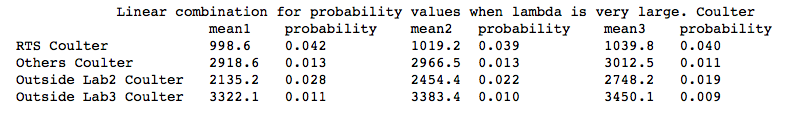
\includegraphics[width=0.9\linewidth]{images/Lambda_Coulter.png}
\caption{Coulter Lambda Values}
\end{figure}

\subsubsection{Discussion of
Assumptions}\label{discussion-of-assumptions}

We discuss the assumptions and tests in bullet points, for brevity.
\begin{itemize}
    \item We felt that the Poisson assumption for the triplet data was given less importance. And the applicability of the model to the data was also not underlined to a desirable extent. One can possibly think of various reasons and situations where doing so is hard to justify. But, beyond our intuition we didn't investigate the validity in detail.
    \item Though one can argue that the parameters fitted to suspected data should not be used to test the validity of the data, we agree with the authors that such a practice only lowers the chances of the suspicion, and gives the person in question a benefit of doubt.
    \item The authors provide a reference for the uniformity of last insignificant digit to a work \cite{mosimann2002terminal}, but fail in explaining why such framework can safely be applied in this context. For instance, there
    might be some characteristics of the underlying biological process which
    prevent the last digits to be uniformly distributed. An attempt to
    clarify and justify this choice in the current setting would have
    beneficial. The authors include here additional data, provided by three
    external sources (two for Coulter counts and one for Colony counts).
    Although the authors comment on the number of these additional samples
    in the Discussion section, we still believe that, in the current
    setting, these additional samples do not help them in making a stronger
    case, but instead can be misleading and add confusion.
    \item As pointed before, we also claim that treating all the other lab
    investigator as a single pool is also not sufficient, since uniformity
    of the pool doesn't necessarily mean of the single contributors. For
    instance, analyzing Table 2 in the paper, it seems that the colony
    counts of the other investigators are even \textit{too good}, having a
    p-value greater than 0.99. We will elaborate more in next sections.


\end{itemize}


\begin{figure}[htbp]
\centering
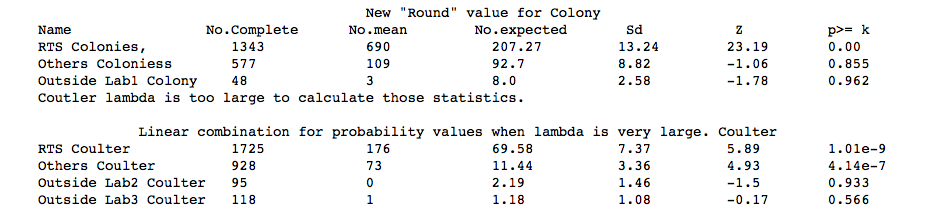
\includegraphics[width=0.9\linewidth]{images/HT_Stat_values.png}
\caption{Approximate Replication of Table 2}
\end{figure}

    \section{Our Analysis}\label{our-analysis}

    The authors begin by singling out that the histogram of RTS looks anomalous
compared to the rest of them put together. They assume that one is
likely to observe uniform distribution for mid-ratio, and this fact is
validated by the histogram of the 9 researchers put together which looks
close to uniform. The first question that came to our mind which motivated this section was - how do we single out the
anomalous researcher if we don't know a priori who he/she is? If we decide on the histogram, then a simple
way would be to plot histograms of the mid-ratios for the data
collected by all researchers individually and look for anomalous patterns
across all these plots. For sake of similarity to the authors' set up,
one will detect anomaly by contrasting each researcher's histogram with
the histogram of all others put together. Such an experiment gives very
interesting results and also raises an important issue with this
approach.
\begin{figure}[H]
\centering
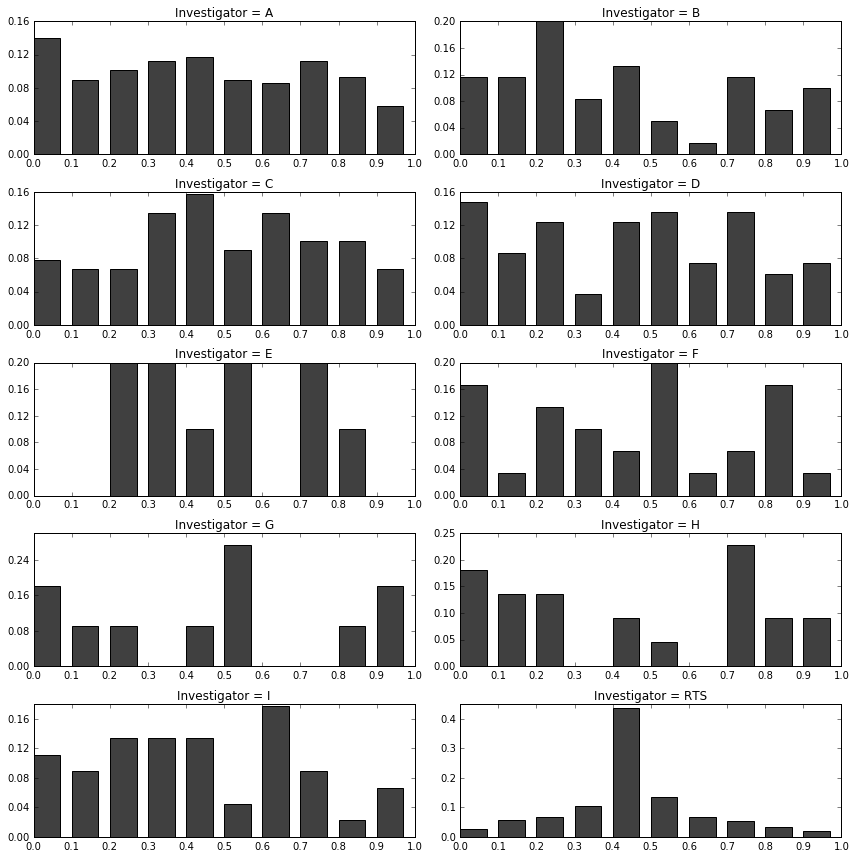
\includegraphics[width=0.8\linewidth]{images/new_mid_ratio.png}
\caption{Individual Histograms for the Colony Data}
\end{figure}

\begin{itemize}
\item
  First, the histogram for researchers with labels ``B, C, E, F, G, H, I'' don't
  seem to be close to uniform as well. In particular, ``B'' and ``C''
  have a very different histogram when contrasted with the histogram for
  uniform distribution. They have distinct peaks but around 0.2 and 0.4
  respectively.
\item
  Second, when we try to contrast the individual histogram of researchers
  with rest of them combined which includes RTS. In the new ``rest''
  histograms, RTS has a dominating effect because of the comparatively
  huge fraction of data collected by RTS, and so most of the other
  researchers look anomalous when contrasted with it.
\end{itemize}

The previous two remarks point out the limitations on the visual
comparison of histogram and assumption of ``uniform distribution'' for
mid ratios. Next we try to present a different viewpoint which has two advantages - it is free of such assumptions, and thus extends to far more general cases where even slight intuition about the data is missing.



    \subsection{Quick Primer to Permutation
Tests}\label{quick-primer-to-permutation-tests}

As discussed above, we felt that the justification for
singling out the particular RTS was incomplete. So, we took a step back,
and did permutation tests to identify anomalous patterns across different
researchers. We briefly discuss the test set up and the philosophy of the test.

Given a treatment and control group of size \(T\) and \(C\)
respectively, we want to test the hypothesis if the treatment has an
effect on the population. In permutation test, the data pooled together
is considered as the population (here it will have size \(N = T+C\)).
Next, one decides on a test statistic that is consistent with our
hypothesis and is expected to contrast the two set of samples if the
treatment has any effect. The distribution of test statistic has an
exact theoretical representation but is often computationally
intractable. An empirical approximation can be made by randomly
partitioning the data into groups of \(T\) and \(C\) several times, and
computing the test statistic contrasting the two datasets. With the
distribution in hand, we can now test how surprising was the outcome
that we originally had.

The conclusion that one draws when the p-values are very low is that \textit{the
two groups are different to each other} than expected had we randomly partitioned
the pooled dataset, i.e., the labels of the data matters.


    \subsection{Permutation Tests for
Mid-Ratio}\label{permutation-tests-for-mid-ratio}

Because we agree with the remark of the authors that it is easy to tweak
the data to get a desirable triplet, we decide to set the difference in
standard deviation of mid-ratios of two datasets. The choice of standard deviation as the first statistic in place of mean
makes sense because uniformity as well as convenient tweaking will lead
to the same expectation of 0.5; and we expect standard deviation to capture
the \textit{unintentional reduction in spread caused in data due to
intentional adjustments}.

We consider each researcher equivalent to a treatment. That is, for a
given researcher, eg. A with dataset \(D_A\) with size \(n_A\), we look
at test statistic computed for a random partition of the entire data
(size \(N\)) into two groups \(n_A\) and \(N-n_A\) and compute the test
statistic. We repeat this experiment 1000 times to plot the empirical
distribution and then compute the p-values. We obtained 0 p-value for A, B,
D, and RTS; and \(<0.01\) p-value for all others except E,F,G which
indicates that almost all datasets are surprising with respect to this
test-statistic. We would like to note that $0$-p value here means that there is less that $1$ in $1000$ chance of observing the event, because of finite resolution owing to $1000$ tests. We would also like to mention that RTS is still the most surprising if one looks at the location of the test-statistic in the
tails of the distribution.

Next we look at \(\ell_1\) distance between the density, followed by
\(\ell_1\) distance between the CDF of two samples for each researcher,
and obtain very similar results as in the previous case, that is several
researchers will be rejected by the test at significance level of even
\(1 \%\). We tabulate all the p-values below.

\begin{figure}[htbp]
\centering
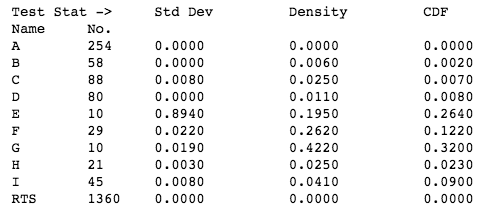
\includegraphics[width=0.8\linewidth]{images/mid_ratio_perm.png}
\caption{Results for Permutation Tests}
\end{figure}

\subsubsection{Limitations of Permutation Test} % (fold)
\label{ssub:limitations_of_permutation_test}

% subsubsection limitations_of_permutation_test (end)
A concern in such a test is the effect of the huge fraction of the data
contributed by RTS. The $p$-values indicate the chance of the difference
between the two groups - treatment and control, so a low $p$-value means
that the treatment group is likely to be different than the control
group. And here the control group has a dominant effect on the data
provided by RTS, hence a heuristic conclusion is that the data of the
other labmates is very different than the data of RTS. To be more
concrete about drawing conclusions about the surprises in data about
other researchers, we exclude the data provided by RTS to run the
permutation tests. We will like to note that this has a bias because we
ignore almost 2/3rd of the data, but doing so does give some answers
that we were expecting before running these tests, which were consistent with the authors' expectations.

\begin{figure}[htbp]
\centering
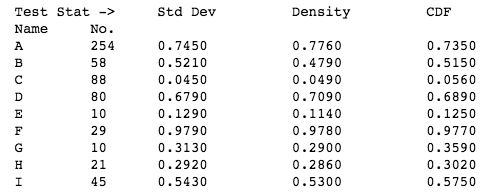
\includegraphics[width=0.8\linewidth]{images/mid_ratio_perm_no_rts.png}
\caption{Results for Permutation Tests without RTS}
\end{figure}

Thus, now the data provided by each individual researchers looks like a
random partitioning when compared to the entire data pooled together
excluding RTS, which gives some statistical evidence to RTS being the
odd one out.

    \subsection{Additional Tests for Digit
Analysis}\label{additional-tests-for-digit-analysis}

One of the main concerns we have had is the decision of the authors to
consider the other investigators as a single pool, instead of performing
additional tests on each of them to show that even taken as single
contributors their data still shows the expected behavior. For the
terminal digit and equal digits tests, we extended the tests provided by
the authors by considering the individual contribution of the single
members of the lab and performing
\begin{itemize}
    \item chi-square test for goodness of fit
for each of the lab members and outside labs for terminal digit analysis,
    \item chi-square test for goodness of fit for each of the lab
members and outside labs for equal digits analysis and,
    \item permutation tests for terminal digit analysis considering RTS and the other investigators.
 \end{itemize}

    \subsubsection{Chi-square test Tests for Terminal Digit
Analysis}\label{chi-square-test-tests-for-terminal-digit-analysis}

To understand how single investigators contributions are distributed
with respect to RTS and the outside labs, we decided to analyze data
from all the other investigators taken one by one. To do so, we
performed the chi-square test for goodness of fit for each of them. The
following tables summarized our results:

\begin{figure}[H]
\centering
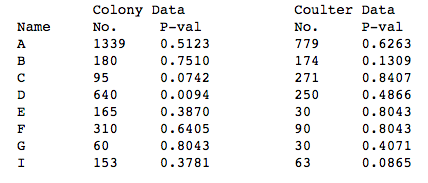
\includegraphics[width=0.7\linewidth]{images/raaz_term_chi_summary.png}
\caption{Chi Square Tests for Terminal Digits in Coulter and Colony
Counts}
\end{figure}

Reading the tables, one can notice that Investigators C and D (for
Coulter counts) and H (for Colony counts) are also quite low if compared
to the others.

    \subsubsection{Chi-square test Tests for Equal Digits
Analysis}\label{chi-square-test-tests-for-equal-digits-analysis}

Also for the Equal Digits Analysis we performed the chi-square test for
goodness of fit using the data of the individual investigators in the
lab, using a similar approach than the Terminal Digit Analysis.
\begin{figure}[H]
\centering
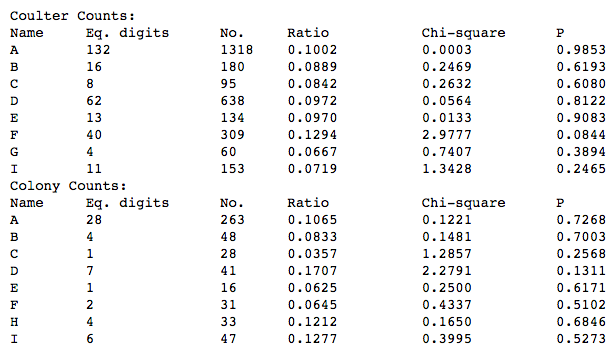
\includegraphics[width=0.9\linewidth]{images/raaz_eq_chi_elaborate.png}
\caption{Chi Square Tests for Equal Terminal Pair in Coulter and Colony
Counts}
\end{figure}

In this case, only investigator F has a relatively low $p$-Value (with respect to
Coulter counts), while investigators A and E have a surprisingly high
$p$-value for the Coulter counts, which might suggest that further
analysis is needed.

    \subsubsection{Permutation Test for Terminal Digit
Analysis}\label{permutation-test-for-terminal-digit-analysis}

The following tables illustrate the permutation test results using the
same test statistics as for mid-ratios:

\begin{figure}[H]
\centering
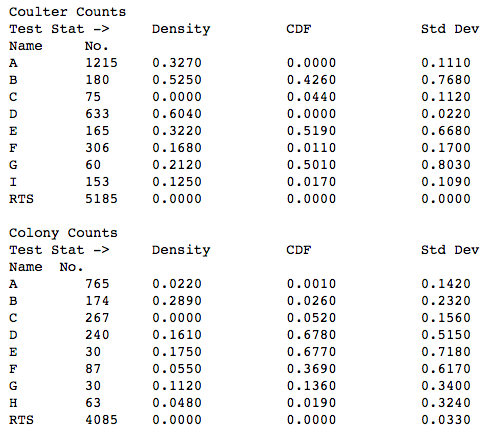
\includegraphics[width=0.7\linewidth]{images/raaz_eq_perm_summary.png}
\caption{Permutation Tests for Terminal Digit Analysis, Coulter counts}
\end{figure}

In all the above cases, it is possible to see how RTS data is
consistently suspicious, which is a confirmation of the authors'
suspects. And as pointed before, the huge fraction of data contributed
by RTS contributes towards the low $p$-values for other individual
researchers as well. We tried permutation tests after excluding RTS data
and get better $p$-values as before, for brevity we do not mention the
values here.

    \section{Conclusion}\label{conclusion}

    Data fraud is an extremely critical issue in science, engineering, and
many other fields. Methods to detect manipulated data are needed to
identify fraudulent research behaviors. Detecting frauds, however, is a
delicate matter. Challenging the credibility of a researcher or of a
scientific work, in fact, can have heavy consequences for all the parties
involved in the process. Methodologies and techniques used in this kind
of work need to be clear and widely accepted, and they need to produce
results which do not leave any space to ambiguity. Independently, reproducibility of
results is a fundamental element to rule out any doubts that could arise
at any time.

In our review, we carefully analyzed the authors' results
and conclusions by reproducing all the results that have been
discussed in the paper and proposing and implementing additional tests to
clarify doubts and suggesting additional directions to the authors.

We found out that authors' results are correct, although it has not been
possible to reproduce exactly all the experiments due to lack of some
key pieces of information (for instance how data has been
pre-processed). Moreover, we encourage the use of stronger tools like permutation tests and our demonstration can be considered as a promotion of the same as such tests helps the analysis to get \textit{rid of assumptions}, thereby shifting the focus from debate on assumptions to actual anomalies present and better understanding of individual
investigator's data, besides the RTS, compares to the general data pool.
At the end of our review, we do believe that there is a significant evidence that RTS has suspicious data, but we suggest the authors to collect additional material and investigate more, since some of our tests suggest that other investigators'
data have anomalies as well if we do not discount the huge fraction of data given by RTS.

\bibliographystyle{apalike}
\bibliography{biblio}

    \end{document}
